%% statlm_paper_en.tex
%% IEEE Conference paper (IEEEtran) -- English version
%% Topic: StatLM -- Zero-shot Multi-Label Vietnamese Text Classification
%%
%% COMPILATION (matches the bundled IEEE conference template toolchain):
%%   pdflatex statlm_paper_en
%%   bibtex   statlm_paper_en
%%   pdflatex statlm_paper_en
%%   pdflatex statlm_paper_en
%% Requires: IEEEtran.cls, IEEEtran.bst and the vntex package (T5 fonts) so that
%% the embedded Vietnamese example labels (e.g., "Giao duc", "Y te") render under
%% pdflatex. If vntex/T5 is unavailable, compile with XeLaTeX/LuaLaTeX and replace
%% the two font lines below with:
%%   \usepackage{fontspec}\setmainfont{TeX Gyre Termes}

\documentclass[conference]{IEEEtran}
\IEEEoverridecommandlockouts
% The preceding line is only needed to identify funding in the first footnote. If
% that is unneeded, please comment it out.

% ---- Unicode + Vietnamese-capable fonts (for the Vietnamese example labels) ----
\usepackage[utf8]{inputenc}
\usepackage[T5]{fontenc}

% ---- Math, tables, figures, citations ----
\usepackage{cite}
\usepackage{amsmath,amssymb,amsfonts}
\usepackage{algorithmic}
\usepackage{graphicx}
\usepackage{textcomp}
\usepackage{xcolor}
\usepackage{booktabs}
\usepackage{array}
\usepackage{multirow}
\usepackage{tabularx}
\usepackage{url}
\def\BibTeX{{\rm B\kern-.05em{\sc i\kern-.025em b}\kern-.08em
    T\kern-.1667em\lower.7ex\hbox{E}\kern-.125emX}}

\interdisplaylinepenalty=2500
\hyphenation{em-bed-ding key-phrase}

\usepackage[hidelinks]{hyperref}

\begin{document}

\title{StatLM: A Hybrid Pipeline for Zero-shot\\
Vietnamese Multi-Label Text Classification}

\author{\IEEEauthorblockN{Tuan Nguyen-Quang}
\IEEEauthorblockA{\textit{VNU - University of Engineering and Technology} \\
Hanoi, Vietnam \\
nqtuan.code@gmail.com}
\and
\IEEEauthorblockN{Trinh Le-Khanh\textsuperscript{*}}
\IEEEauthorblockA{\textit{VNU - University of Engineering and Technology} \\
Hanoi, Vietnam \\
trinhlk@vnu.edu.vn}
\thanks{*Corresponding author: Trinh Le-Khanh (e-mail: trinhlk@vnu.edu.vn)}

}

\maketitle

\begin{abstract}
The rapid growth of digital documents has increased the need for scalable document organization across languages and domains.
Open-world zero-shot multi-label text classification is challenging because neither the label space nor the document-level labels are specified in advance, and task-specific labeled data are unavailable. Existing approaches typically trade off label-space quality, large language model (LLM) usage, and processing time. This paper presents \textbf{StatLM}, a hybrid pipeline that combines a statistical encoder with an LLM decoder. The encoder first applies extractive TextRank using Vietnamese sentence embeddings and then uses KeyBERT with an asymmetric retrieval model to represent each document by a compact set of keyphrases. The LLM is invoked only at the final decoder stage to construct and normalize the label space and to assign labels. On a balanced VietnamNet corpus of 2{,}000 articles from 20 categories, StatLM increases the coarse-label ratio from 32.6\% to 76.9\%, reduces the noise-label ratio from 39.1\% to 3.8\%, and covers 19 of 20 categories, compared with 15 of 20 for X-MLClass-Gemini, our full-LLM baseline that follows the X-MLClass pipeline with Gemini 2.5 Flash as the backbone. StatLM also reduces the mean processing time from 40 to 10 seconds per document, uses approximately $30$ times fewer LLM tokens, and requires one API call rather than approximately eight. These results indicate that statistical noise reduction and content condensation before LLM-based label generation provide a favorable quality, efficiency trade-off for resource-constrained deployment.
\end{abstract}

\begin{IEEEkeywords}
Coarse labeling, hybrid pipeline, KeyBERT, large language model, statistical
encoder, StatLM, TextRank, Vietnamese natural language processing, zero-shot
multi-label text classification.
\end{IEEEkeywords}

% ============================================================
\section{Introduction}
% ============================================================
The volume of Vietnamese digital text from online news, electronic commerce,
social media, and academic repositories continues to grow, making manual document
organization increasingly difficult. This study considers \emph{open-world
zero-shot multi-label text classification}, in which a system must infer the label
space and assign one or more labels to each document without task-specific labeled
data or a predefined label inventory~\cite{li2024open}. In this setting, the label
space may be expanded as additional document batches are processed. Such a capability is relevant to document collections for which a fixed taxonomy is unavailable or expensive to maintain.
Existing methods can be broadly grouped into three categories~\cite{li2024open}.
Supervised classifiers can achieve high predictive accuracy when a complete label
set and sufficient labeled examples are available, but these assumptions do not
hold in the target setting. Direct LLM-based methods can generate labels from raw
text without task-specific training, but repeated processing of long documents
increases token usage and latency and may produce entity-level or overly specific
labels. Statistical methods, including topic modeling and keyphrase extraction,
are computationally efficient but generally return topics or phrases rather than a
normalized, human-readable multi-label taxonomy. These limitations motivate a
method that combines statistical filtering with LLM-based semantic generalization.

We propose \emph{StatLM}, a pipeline comprising a statistical encoder and an LLM
decoder. The encoder removes low-centrality content and represents each document by
a compact, diverse set of keyphrases. The decoder then uses these representations
to discover, normalize, and assign coarse-grained labels. Restricting LLM processing to the final stage is intended to retain the semantic flexibility of generative models while reducing exposure to raw-text noise and limiting API usage.

The contributions of this work are as follows. First, we formulate a
hybrid encoder-decoder architecture for open-world zero-shot multi-label
classification and position it relative to supervised, statistical, and direct
LLM-based alternatives. Second, we develop a Vietnamese processing pipeline that
uses embedding-based TextRank for extractive summarization and configures KeyBERT
with an asymmetric retrieval model for keyphrase extraction. Third, we construct
and release a balanced VietnamNet corpus and evaluate the proposed pipeline at the
summarization, keyphrase-extraction, label-space, classification, and computational
levels against statistical baselines and an X-MLClass-based full-LLM baseline.

The remainder of this paper is organized as follows. Section~\ref{sec:related}
reviews the relevant methods and Vietnamese language resources.
Section~\ref{sec:method} describes the StatLM architecture, and
Section~\ref{sec:setup} presents the dataset, baselines, and evaluation protocol.
Section~\ref{sec:results} reports and discusses the experimental results.
Section~\ref{sec:conclusion} summarizes the findings, limitations, and directions
for future work.


% ============================================================
\section{Background and Related Work}
\label{sec:related}
% ============================================================

\subsection{Graph-Based Extractive Summarization}
Extractive summarization preserves source wording and requires no summary-specific
training data. Graph-based methods represent sentences as nodes and their relations
as weighted edges, then estimate sentence importance from the graph structure.
TextRank applies PageRank to this representation~\cite{mihalcea2004textrank}, but
its performance depends on the edge-weight function. Word overlap and variants
based on TF-IDF, LexRank, BM25+, or LDA-extended TextRank primarily capture lexical
relations~\cite{vora2024extractive}. Sentence embeddings instead model semantic
similarity between lexically different sentences~\cite{kadriu2021extractive}.

\subsection{Keyphrase Extraction}
Unsupervised keyphrase extraction includes statistical methods such as RAKE
~\cite{rose2010automatic} and YAKE~\cite{campos2020yake}; graph-based methods such
as TextRank~\cite{mihalcea2004textrank}, TopicRank~\cite{bougouin2013topicrank},
MultipartiteRank~\cite{boudin2018unsupervised}, and WordAttractionRank
~\cite{wang2014corpus}; and embedding-based methods. KeyBERT
~\cite{grootendorst2020keybert} ranks candidate n-grams by cosine similarity to the
document and can apply maximal marginal relevance (MMR)~\cite{carbonell1998use} to
reduce redundancy. Here, matching a short phrase to a document summary is an
asymmetric retrieval task; a retrieval-oriented embedding model is therefore more
appropriate than one optimized only for symmetric semantic textual similarity
(STS).

\subsection{Label-Space Discovery}
Label-space discovery has used topic models, embedding-and-clustering methods, and
LLM-assisted topic naming. Many such pipelines assume a fixed topic count or a
single dominant topic per document. X-MLClass~\cite{li2024open} uses an LLM for
chunking, keyphrase generation, clustering, and iterative rare-label discovery.
However, repeated raw-text processing increases token usage and latency and may
produce entity-level or journalistic labels on news data. StatLM instead places a
statistical encoder before the LLM so that label discovery operates on condensed
keyphrases.

\subsection{Vietnamese Processing Resources}
StatLM uses pyvi~\cite{pyvi} for word segmentation and VnCoreNLP
~\cite{vu2018vncorenlp} for segmentation, part-of-speech (POS) tagging, and
named-entity recognition (NER). The encoder models are matched to their tasks
(Table~\ref{tab:emb}). \emph{dangvantuan/vietnamese-embedding}
~\cite{dangvantuan2021vietnamese}, a Sentence-BERT model
~\cite{reimers2019sentence} based on PhoBERT~\cite{nguyen2020phobert}, is optimized
for symmetric STS and reports Pearson 84.21 on \emph{vi-stsbenchmark}.
\emph{bkai-foundation-models/vietnamese-bi-encoder}
~\cite{nguyen2025improving} is trained for asymmetric retrieval and is reported to
rank first on the Vietnamese VCS benchmark.


% ============================================================
\section{The StatLM Method}
\label{sec:method}
% ============================================================
StatLM uses the three-layer encoder-decoder architecture in Fig.~\ref{fig:arch}.
Two encoder layers summarize each document and extract keyphrases; the LLM decoder
then constructs the label space and assigns labels. New batches are matched to the
existing label space, while unmatched documents form new clusters. Although the
linguistic tools and embeddings are pretrained, no domain-specific labeled data are
used for label discovery or classification.

\begin{figure*}[!t]
\centering
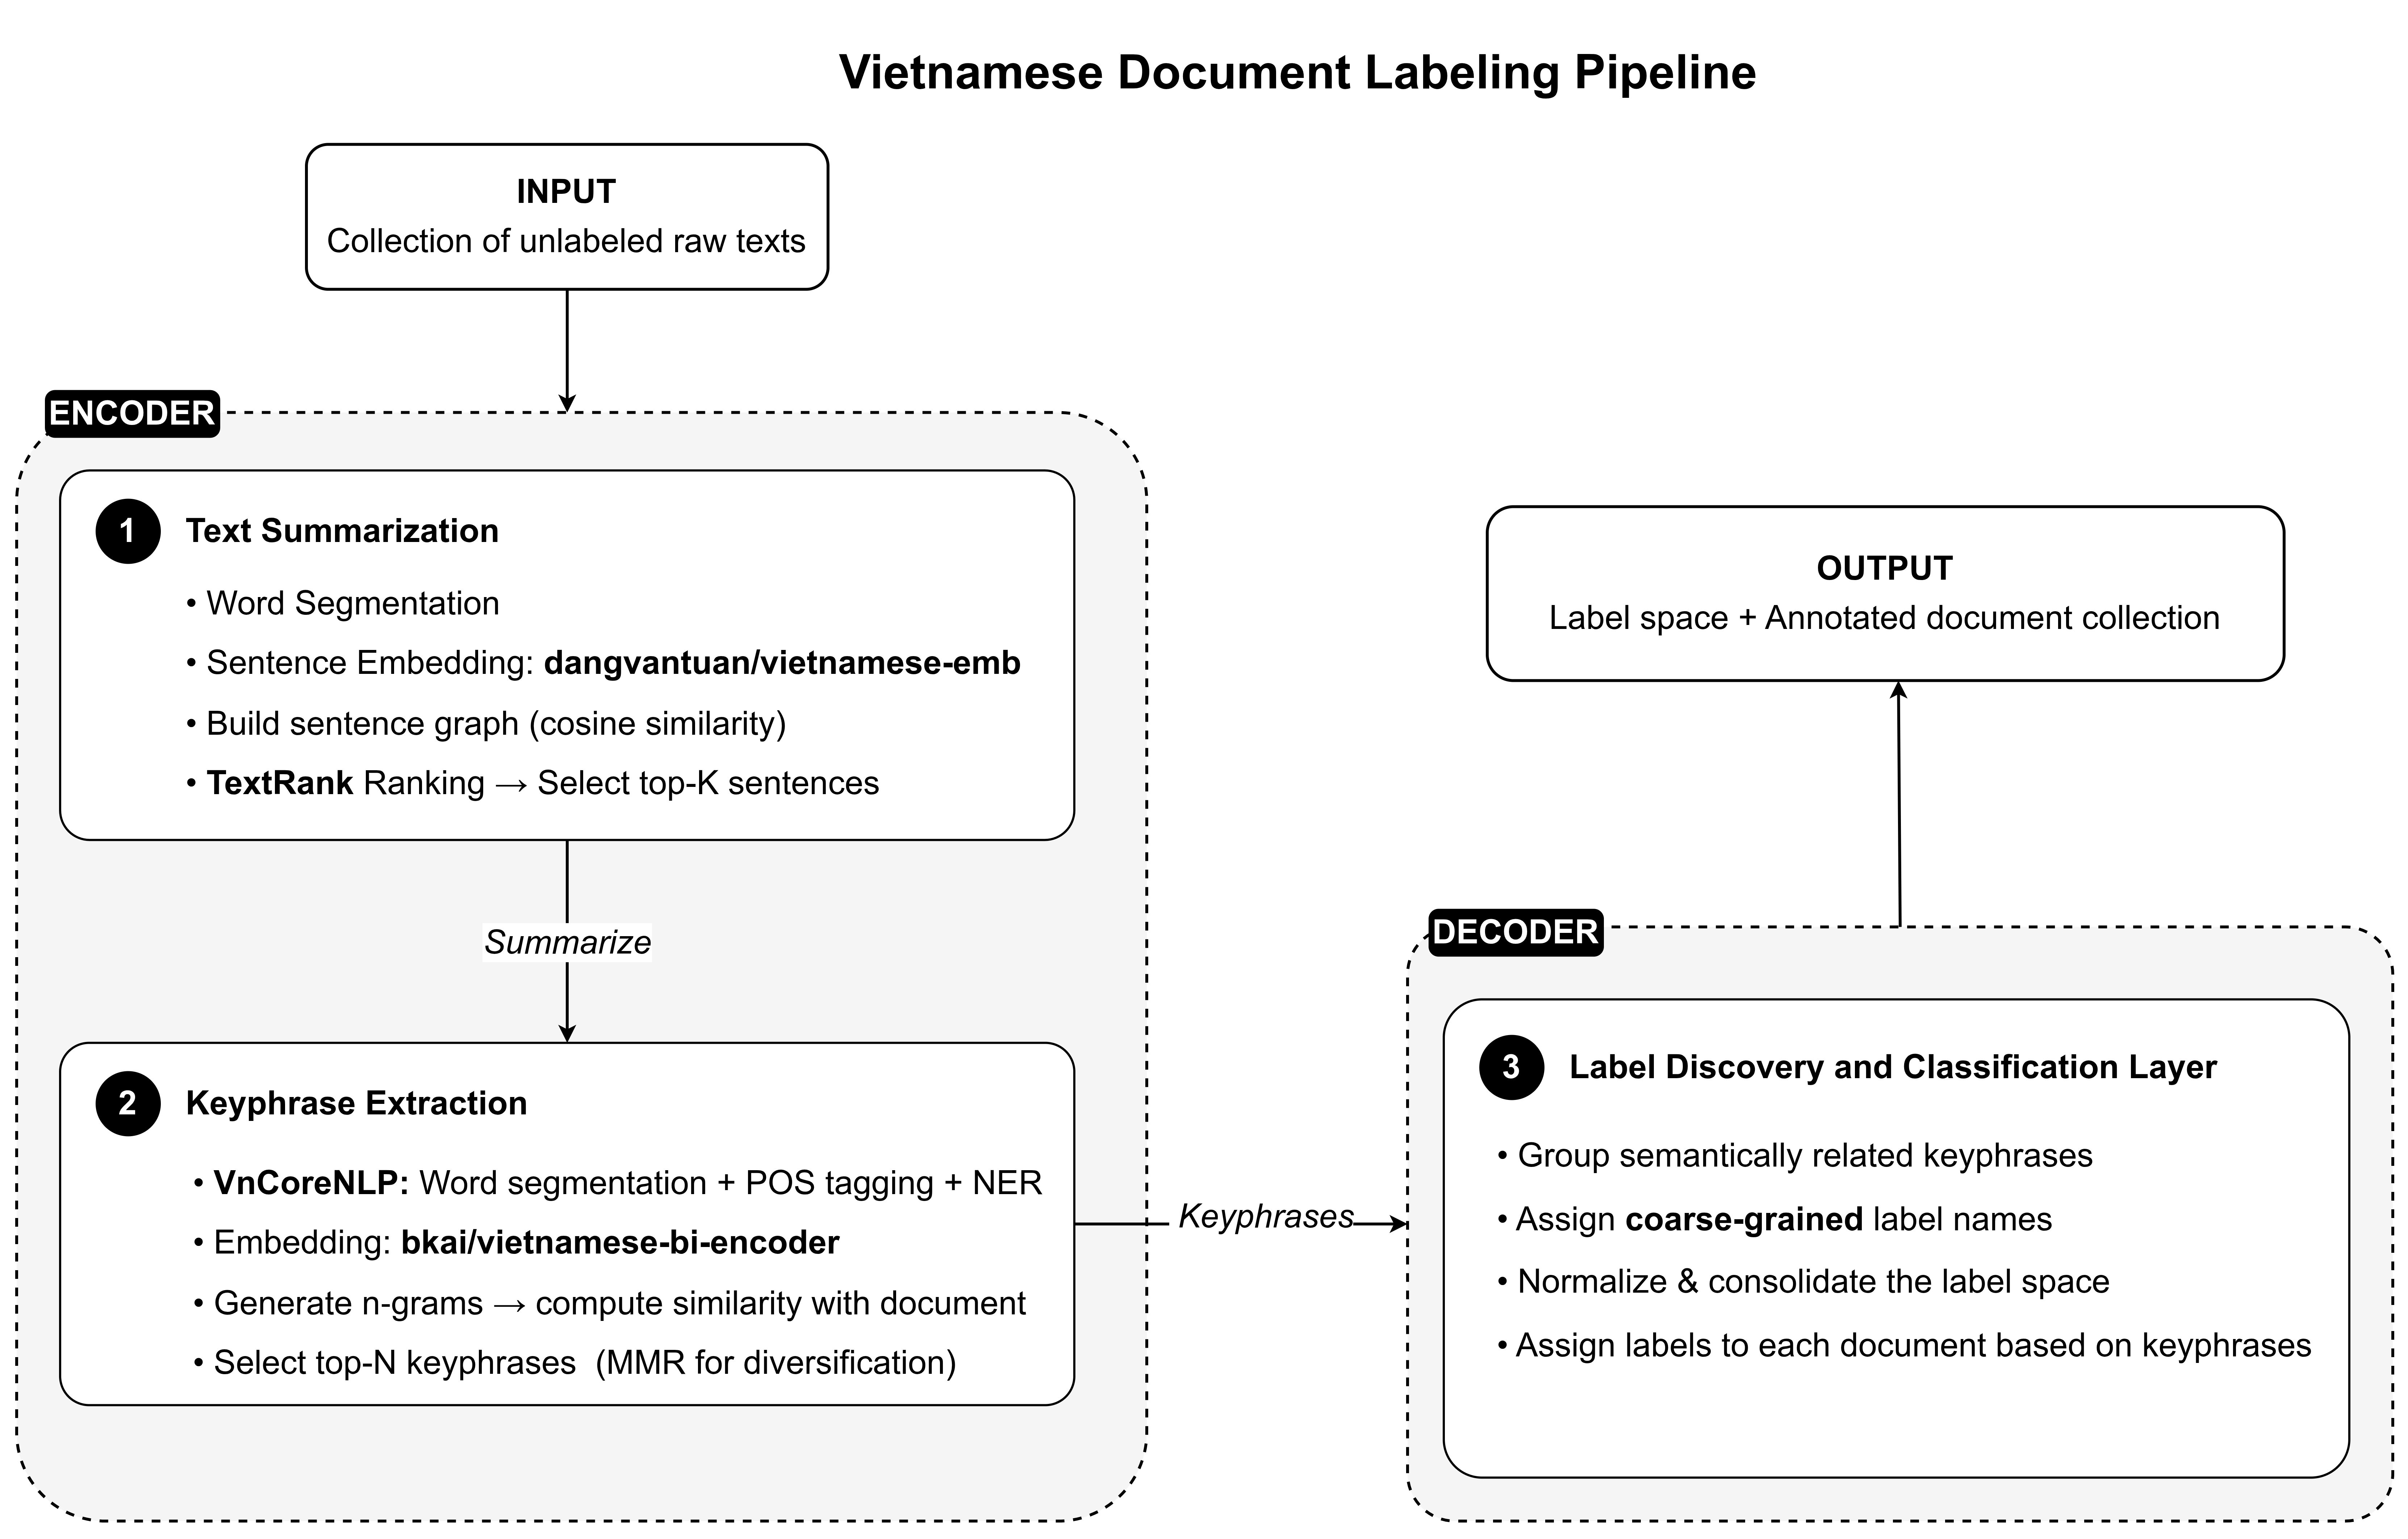
\includegraphics[width=0.93\textwidth]{figures/overview.png}
\caption{StatLM architecture: two statistical encoder layers condense each
document before the LLM decoder constructs, normalizes, and assigns labels.}
\label{fig:arch}
\end{figure*}
% \begin{figure*}[!t]
% \centering
% 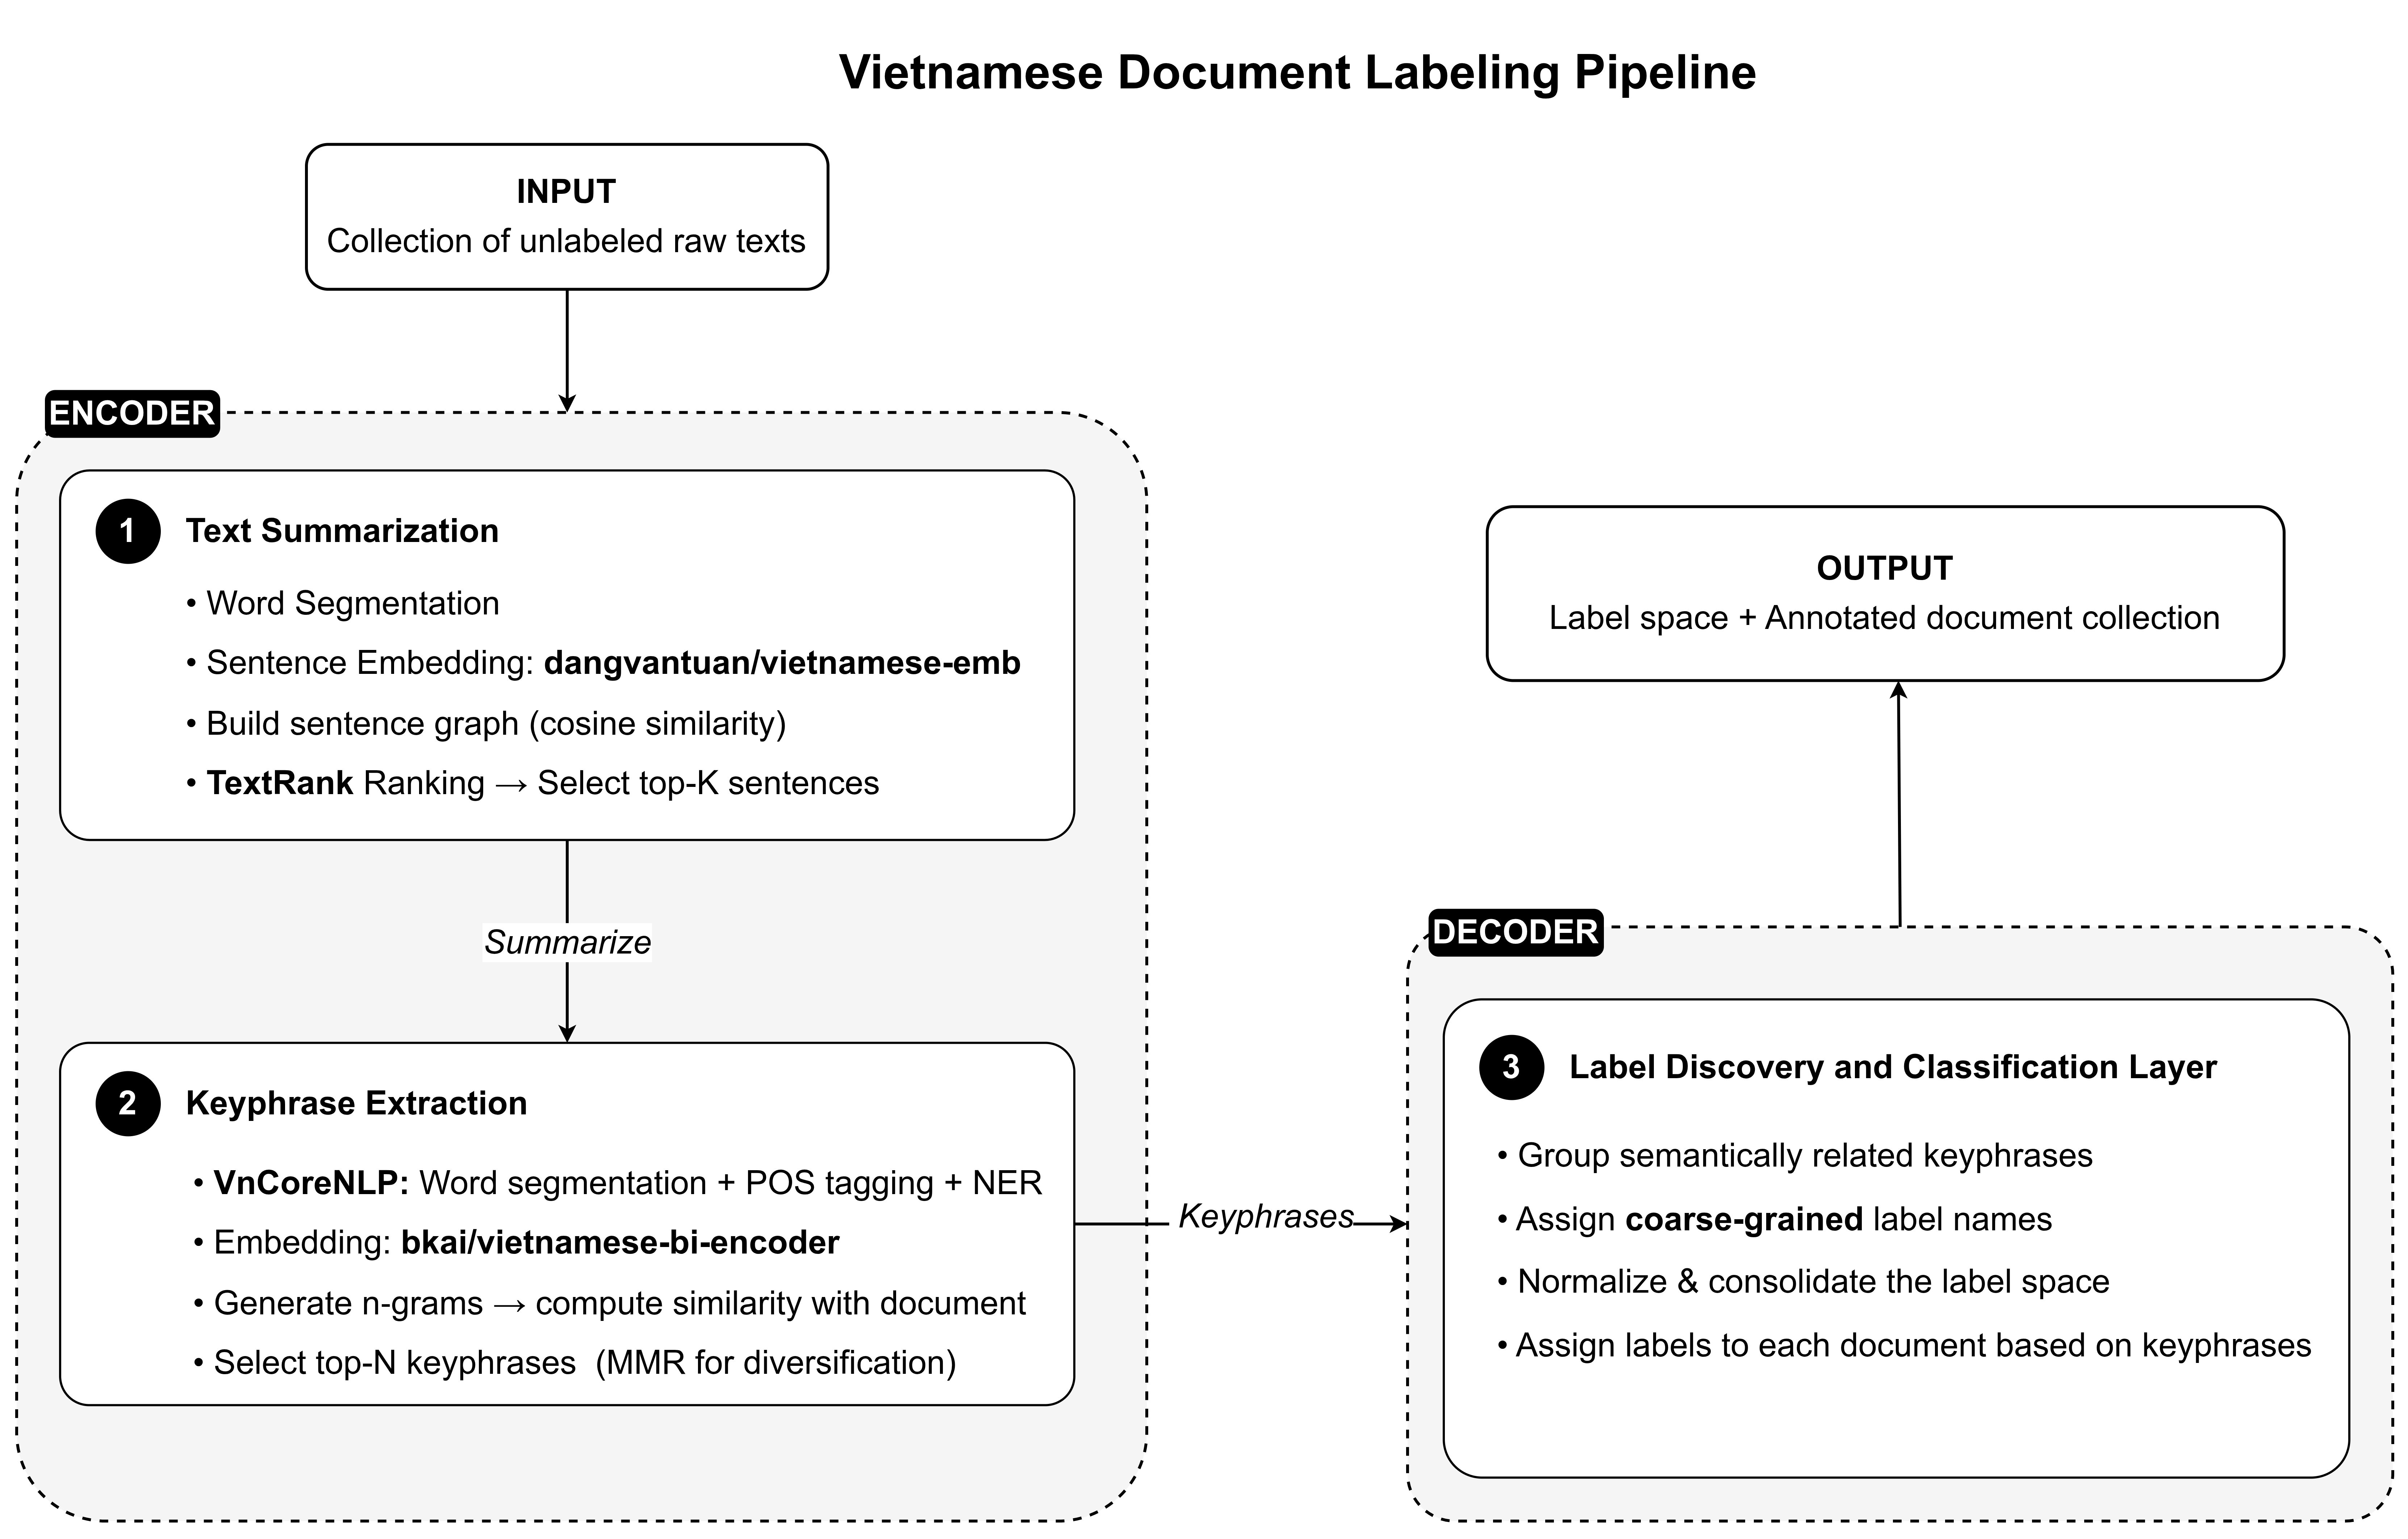
\includegraphics[width=0.95\textwidth]{figures/overview.png}
% \caption{Overall architecture of StatLM: the statistical encoder has two layers
% (summarization with TextRank + \emph{dangvantuan/vietnamese-embedding}; keyphrase
% extraction with KeyBERT + \emph{bkai/vietnamese-bi-encoder} and VnCoreNLP) that
% reduce noise and condense the information; the LLM decoder (Gemini) is invoked
% only once at the end to discover, name, and normalize the label space and to
% assign labels to each document.}
% \label{fig:arch}
% \end{figure*}

\subsection{Layer 1: Text Summarization}
For document $D=\{s_1,\ldots,s_n\}$, Layer~1 produces summary
$S=\{s'_1,\ldots,s'_k\}$, where $k<n$. StatLM applies TextRank with semantic edge
weights rather than word overlap or other lexical similarities. Because the layer
compares sentences of similar length, it uses the symmetric-STS model
\emph{dangvantuan/vietnamese-embedding}~\cite{dangvantuan2021vietnamese} with pyvi
preprocessing.

The document is split into sentences and segmented with pyvi. Each sentence is
encoded as $\mathbf{e}_i=\mathrm{meanpool}(\mathrm{PhoBERT}(s_i))\in
\mathbb{R}^{768}$, and a complete graph is built with
$W_{ij}=\cos(\mathbf{e}_i,\mathbf{e}_j)$. TextRank computes
\begin{equation}
\begin{aligned}
\mathrm{WS}(v_i)^{(t+1)} &=(1-d)+d\!\!\sum_{v_j\in\mathrm{In}(v_i)}
\frac{w_{ji}}{\sum_{v_k\in\mathrm{Out}(v_j)}w_{jk}}\\
&\quad\times\mathrm{WS}(v_j)^{(t)},
\end{aligned}
\label{eq:textrank}
\end{equation}
with $d=0.85$ and convergence threshold $\varepsilon=10^{-5}$. For $n>5$, the
$k=\max(5,\lceil0.4n\rceil)$ highest-ranked sentences are retained and restored to
their original order.

\begin{figure}[!t]
\centering
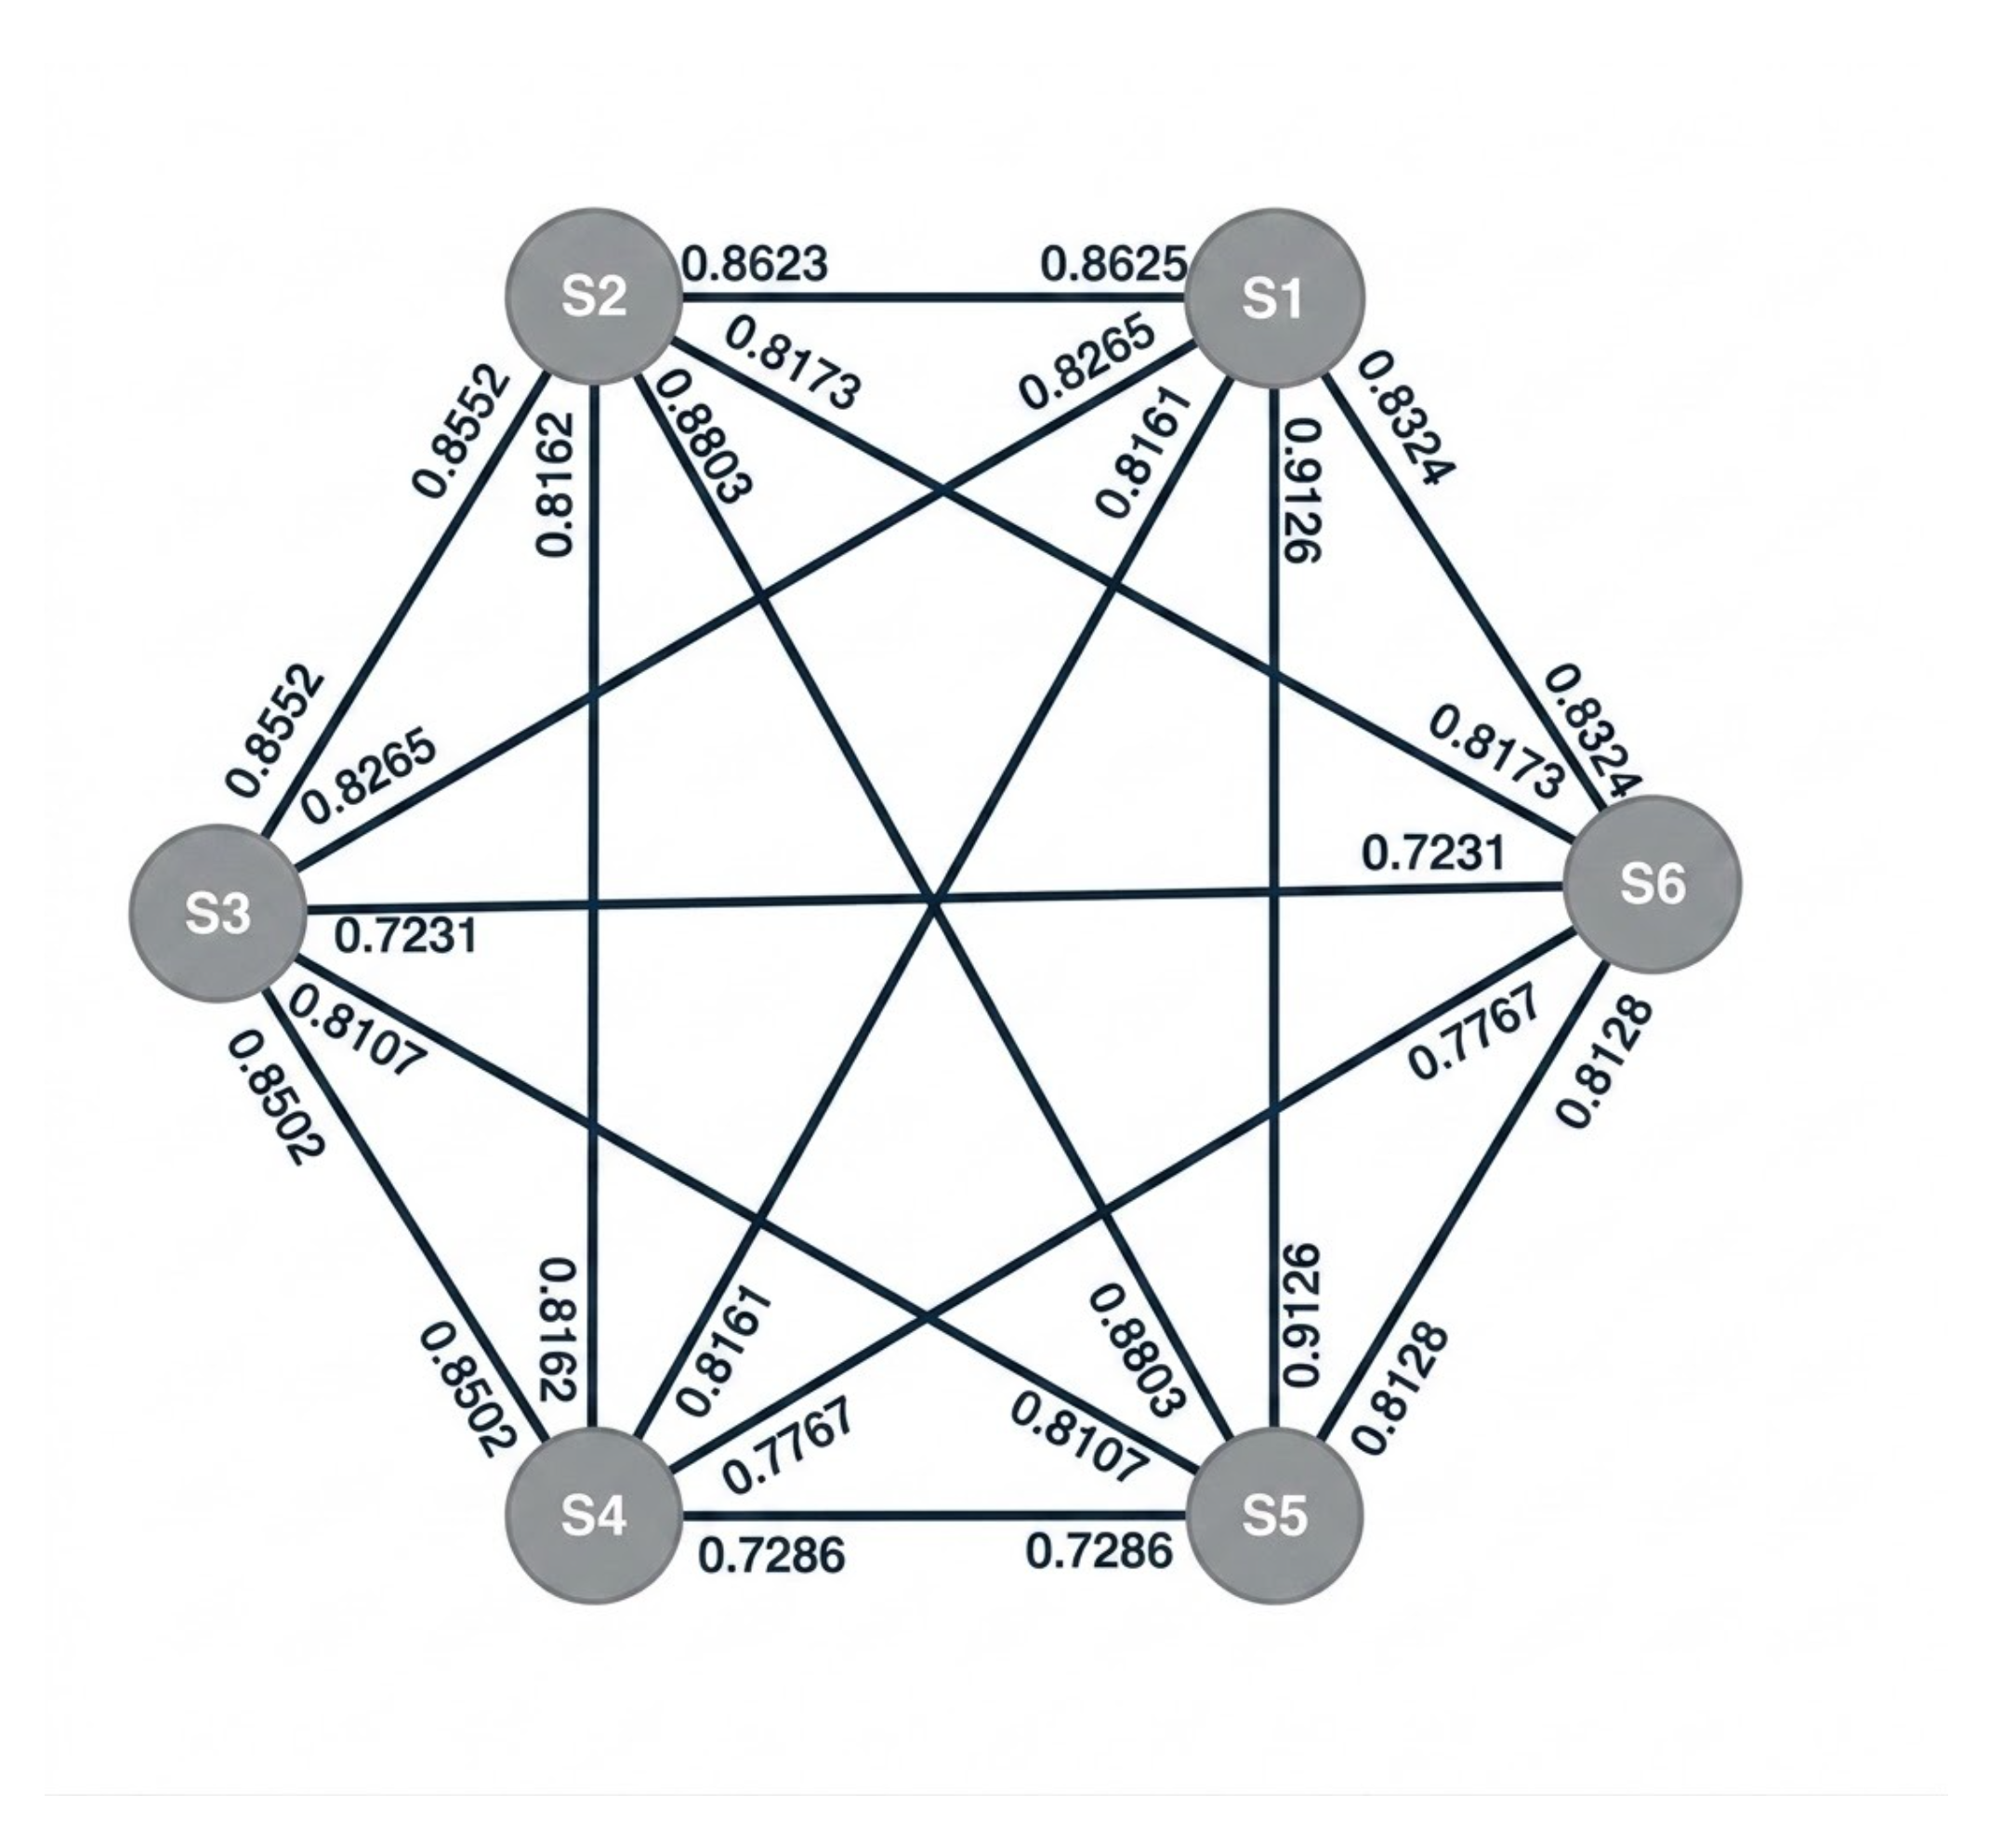
\includegraphics[width=0.95\columnwidth]{figures/stage1.png}
\caption{Layer~1 ranks a semantic sentence graph with TextRank and retains the
top-$k$ sentences.}
\label{fig:textrank}
\end{figure}

The canonical PageRank/TextRank value is fixed as $d=0.85$ because the $(1-d)$ teleportation term only keeps the walk ergodic and the ranking is documented to be insensitive to $d$ over $[0.8,0.9]$. Dataset-specific fusion schemes
~\cite{vora2024extractive} are omitted so that the retention ratio $r$ remains the
principal Layer~1 parameter. 

A sentence's score accumulates its weighted semantic similarity to the rest of the document, so the roughly 60\% discarded are low-centrality nodes such as redundant restatements, transitions, boilerplate, or peripheral asides. A recurring main subject is effectively preserved, whereas a secondary subject confined to a few low-centrality sentences may fall below the cut and cannot be recovered downstream. A sweep over $r\in[0.2,0.6]$ (Table~\ref{tab:retention}) shows closeness to the title-and-SAPO lead decreasing while topical coverage rises, so the proportional budget $k=\max(5,\lceil0.4n\rceil)$ is adopted, consistent with embedding-based TextRank outperforming Lead-$K$ on ROUGE (Table~\ref{tab:rouge}).


\subsection{Layer 2: Keyphrase Extraction}

Layer~2 extracts $m=10$ one-to-three-word keyphrases from $S$ using KeyBERT
~\cite{grootendorst2020keybert} and the asymmetric retrieval model
\emph{bkai-foundation-models/vietnamese-bi-encoder}
~\cite{nguyen2025improving}. VnCoreNLP~\cite{vu2018vncorenlp} supplies POS tags and
NER spans. Candidate n-grams are generated within sentence boundaries, filtered by
stopwords and POS tags, and supplemented with complete named-entity spans.

The procedure is: (1) preprocess with VnCoreNLP, remove stopwords, and filter by POS; (2) encode the summary into $\mathbf{E}_{doc}$; (3) generate one-to-three-word candidate n-grams within sentence fragments, adding NER entities; (4) compute
\begin{equation}
\cos(\mathbf{E}_{doc},\mathbf{E}_{ngram})=
\frac{\mathbf{E}_{doc}\cdot\mathbf{E}_{ngram}}
{\lVert\mathbf{E}_{doc}\rVert\,\lVert\mathbf{E}_{ngram}\rVert};
\label{eq:cosine}
\end{equation}
and (5) select keyphrases with MMR~\cite{carbonell1998use}:
\begin{equation}
\mathrm{MMR}=\arg\max_{c\notin S}\Big[\lambda\,\mathrm{sim}(c,doc)
-(1-\lambda)\max_{s\in S}\mathrm{sim}(c,s)\Big],
\label{eq:mmr}
\end{equation}
with $\lambda=0.5$ and redundancy cap $\theta=0.7$. The neutral midpoint is used because the top-5 keyphrases must jointly span a document's facets: emphasizing relevance yields near-duplicates, whereas emphasizing diversity admits loosely related phrases that become decoder noise. The hard cap removes a candidate whose cosine to an already selected phrase exceeds $\theta$, preserving adjacent facets while suppressing paraphrases and head-sharing substrings. With POS- and NER-filtered candidates, selection is stable around $(\lambda,\theta)=(0.5,0.7)$.

\begin{figure*}[!t]
\centering
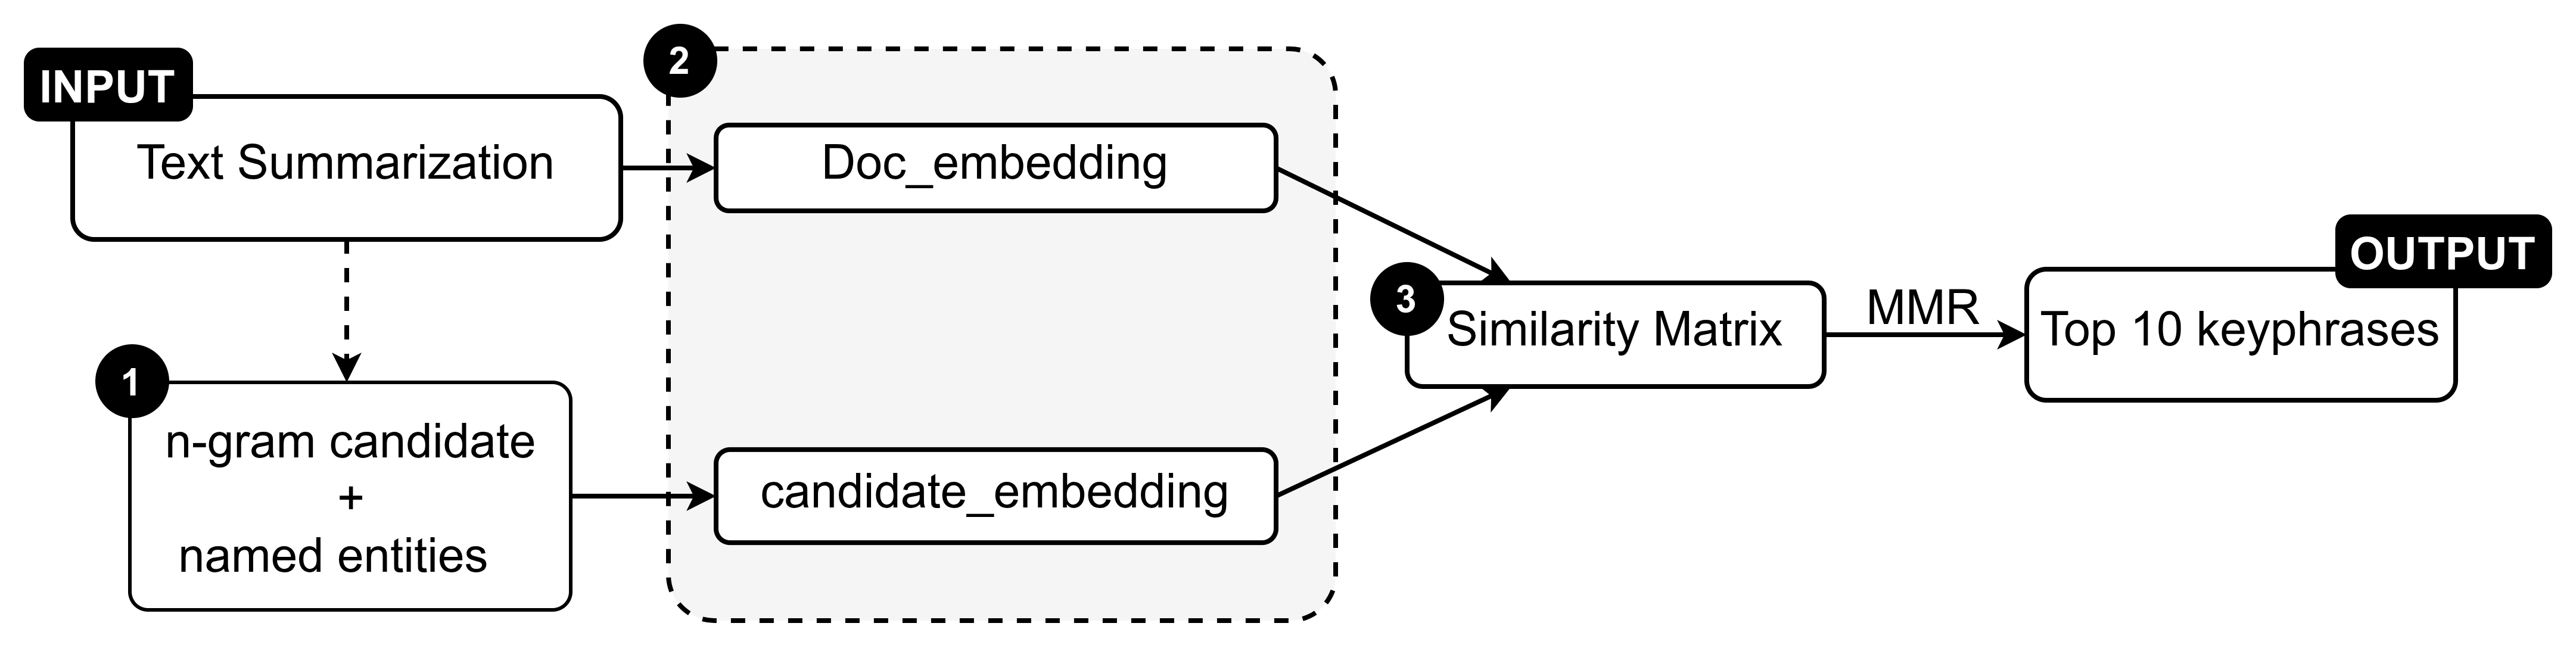
\includegraphics[width=0.8\textwidth]{figures/stage2.png}
\caption{Layer~2 encodes the summary and candidate n-grams independently, then
uses cosine ranking and MMR to select diverse keyphrases.}
\label{fig:keybert}
\end{figure*}

\begin{table}[!t]
\renewcommand{\arraystretch}{1.25}
\caption{Embedding Models Used by the Two Encoder Layers}
\label{tab:emb}
\centering
\scriptsize
\begin{tabularx}{\columnwidth}{@{}lXX@{}}
\toprule
\textbf{Criterion} & \textbf{Layer 1 (TextRank)} & \textbf{Layer 2 (KeyBERT)} \\
\midrule
Problem type & Symmetric STS & Asymmetric retrieval \\
Relation     & Sentence to sentence & Keyphrase to document \\
Model        & dangvantuan embedding & bkai bi-encoder \\
Tokenizer    & pyvi & VnCoreNLP \\
Score        & Pearson 84.21 & First on VCS retrieval \\
\bottomrule
\end{tabularx}
\end{table}

\subsection{Layer 3: Classification and Labeling with the LLM}
Given the keyphrase set $\mathcal{P}=\{p_1,\dots,p_N\}$ of $N$ documents, this layer discovers the label space $\mathcal{L}=\{l_1,\dots,l_M\}$ and assigns labels. StatLM places Gemini 2.5 Flash at the decoder after filtering and condensation, so far fewer tokens reach the API and source entities or formatting are less likely to induce noisy labels. It supports new and incremental data in three steps: (1) send only the top-5 keyphrases per document for normalization; (2) assign documents to existing clusters under a strict policy, allowing label-rename suggestions and routing non-matches to an ``unassigned'' list; and (3) cluster and name the unassigned documents. A System Message requests coarse-grained labels, avoids entity-like labels (e.g., ``Giáo dục''/``Education'' rather than ``Tuyển sinh đại học 2024''/``University Admissions 2024''), minimizes label count, and merges similar topics.



% ============================================================
\section{Experimental Setup}
\label{sec:setup}
% ============================================================
Experiments use the \emph{VietnamNet} dataset: 2{,}000 news articles evenly spread over 20 categories (100 each), each 500--800 words with a title, lead paragraph (\emph{sapo}), and keyphrase list. All three tasks are evaluated on the full corpus. References differ by task: title + sapo for summarization; an LLM-generated keyphrase list (DeepSeek~V4) for keyphrase extraction~\cite{pavlovic2024effectiveness}; and the 20 original categories as a coarse-label proxy, because no absolute label-space ground truth exists~\cite{wan2024tnt}.

All runs use a personal machine (12th-generation Intel Core i7, 16~GB RAM, no GPU); embeddings run on CPU through \texttt{sentence-transformers}, and the LLM through the Google API. Fixed parameters are: Layer~1 $d=0.85$, $\varepsilon=10^{-5}$, 40\% retention (minimum five sentences); Layer~2 one-to-three-word n-grams, $m=10$, $\lambda=0.5$; and Layer~3 \texttt{gemini-2.5-flash} with temperature 0.1 for classification and 0.3 for label generation, sending at most five keyphrases per document.


\emph{Baselines.} Summarization uses Lead-$K$, word-overlap TextRank, and
TextRank+TF--IDF. Keyphrase baselines are RAKE, YAKE, TextRank-keywords, TopicRank,
MultipartiteRank, WordAttractionRank, and KeyBERT with a symmetric embedding. The
end-to-end \emph{X-MLClass-Gemini} baseline follows X-MLClass~\cite{li2024open} using
50-token chunks, four keyphrases per chunk, BERTopic, NLI entailment, and ten
long-tail iterations. We denote the adapted baseline as X-MLClass-Gemini because it
follows the X-MLClass pipeline while replacing the original LLM with Gemini 2.5 Flash
for backbone comparability.

\emph{Metrics.} Summarization uses ROUGE-1/2/L F1. Keyphrase extraction uses
precision, recall, and F1 at $k=5$ and 10 with exact or soft matching
(cosine $\geq0.7$). Discovered labels are classified as Coarse, Long-tail, Entity,
Meta/Noise, or Cross-topic, yielding the Coarse ratio, Noise ratio, and category
coverage. End-to-end ranking is measured by
\begin{equation}
P@k = \frac{1}{N}\sum_{i=1}^{N}
\frac{\lvert C_i^{rk}\cap L_i\rvert}{\min(k,\lvert L_i\rvert)},
\label{eq:pak}
\end{equation}
where $C_i^{rk}$ is the top-$k$ prediction and $L_i$ is the reference set. Since
$\lvert L_i\rvert=1$, the measure reduces to top-$k$ accuracy under this proxy.



% ============================================================
\section{Results and Discussion}
\label{sec:results}
% ============================================================

\subsection{Summarization Evaluation (Layer 1)}
Embedding-based TextRank obtains the highest ROUGE scores
(Table~\ref{tab:rouge}). Relative to word-overlap TextRank, ROUGE-1 F1 increases by
approximately 18\% (0.341 to 0.403), and ROUGE-2 F1 increases by approximately
22\% (0.162 to 0.198). The results support semantic rather than lexical edge
weights for the sentence graph.

\begin{table}[!t]
\renewcommand{\arraystretch}{1.2}
\caption{Summarization ROUGE F1 Scores on VietnamNet}
\label{tab:rouge}
\centering
\footnotesize
\begin{tabularx}{\columnwidth}{@{}Xccc@{}}
\toprule
\textbf{Method} & \textbf{ROUGE-1} & \textbf{ROUGE-2} & \textbf{ROUGE-L} \\
\midrule
Lead-K ($k=5$)              & 0.312 & 0.145 & 0.283 \\
Original TextRank           & 0.341 & 0.162 & 0.307 \\
TextRank + TF-IDF           & 0.358 & 0.171 & 0.324 \\
\textbf{TextRank + embedding}   & \textbf{0.403} & \textbf{0.198} & \textbf{0.371} \\
\bottomrule
\end{tabularx}
\end{table}

Sweeping $r\in[0.2,0.6]$ (Table~\ref{tab:retention}), semantic closeness to the title+sapo lead (SemSim) falls while topical coverage (KP-Cov) rises. Both coverage and token cost grow with $r$, so $r=0.4$ is a balanced operating point: it retains sufficient coverage for open-world discovery without inflating the LLM token load.


\begin{table}[!t]
\renewcommand{\arraystretch}{1.2}
\caption{Layer-1 retention sweep; $r{=}0.4$ balances lead similarity and topical coverage}
\label{tab:retention}
\centering
\footnotesize
\begin{tabular*}{\columnwidth}{@{\extracolsep{\fill}}cccc@{}}
\toprule
\shortstack{Retention\\ratio $r$} & \shortstack{Compression\\ratio}
 & \shortstack{Semantic\\similarity $\downarrow$}
 & \shortstack{Keyphrase\\coverage $\uparrow$} \\
\midrule
0.20 & 0.39 & 0.510 & 0.266 \\
0.25 & 0.41 & 0.506 & 0.275 \\
0.30 & 0.45 & 0.501 & 0.287 \\
0.35 & 0.49 & 0.496 & 0.298 \\
\textbf{0.40} & \textbf{0.53} & \textbf{0.490} & \textbf{0.306} \\
0.45 & 0.57 & 0.483 & 0.316 \\
0.50 & 0.61 & 0.477 & 0.324 \\
0.55 & 0.66 & 0.470 & 0.334 \\
0.60 & 0.70 & 0.464 & 0.340 \\
\bottomrule
\end{tabular*}
\end{table}

% \begin{figure}[!t]
% \centering
% 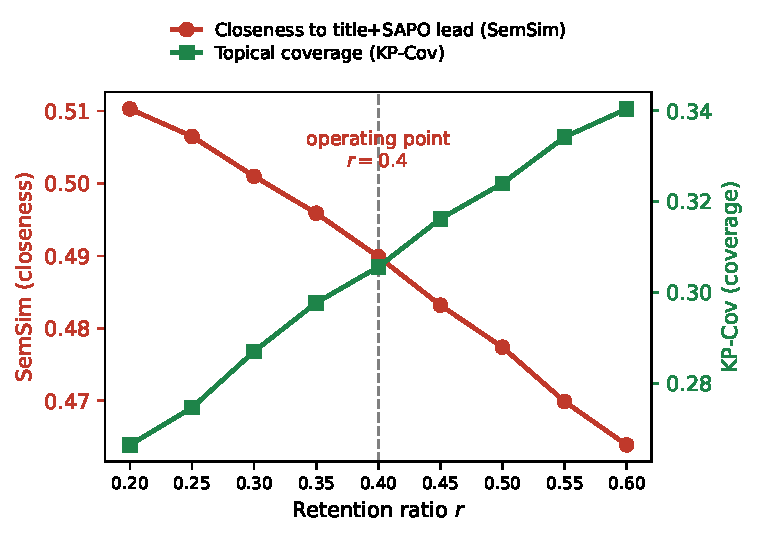
\includegraphics[width=0.92\columnwidth]{figures/retention_balance.pdf}
% \caption{Trade-off over the retention ratio $r$: closeness to the title-and-SAPO lead
% (SemSim, left axis) falls while topical coverage (KP-Cov, right axis) rises. The
% value $r{=}0.4$ is adopted as the operating point.}
% \label{fig:retention}
% \end{figure}

\subsection{Keyphrase-Extraction Evaluation (Layer 2)}
StatLM's KeyBERT leads on every metric (Table~\ref{tab:keyphrase}). The gap between the two KeyBERT variants (F1@10: 30.10 vs. 25.51, about 18\%) confirms the role of \emph{asymmetric embedding} in bridging short keyphrases and long documents. WordAttractionRank leads the graph group (F1@10 = 25.21) but trails KeyBERT because it lacks a redundancy mechanism such as MMR.

\begin{table}[!t]
\renewcommand{\arraystretch}{1.2}
\caption{Keyphrase-Extraction Results on VietnamNet (in \%)}
\label{tab:keyphrase}
\centering
\scriptsize
\setlength{\tabcolsep}{4pt}
\begin{tabular}{@{}lcccccc@{}}
\toprule
\textbf{Method} & \textbf{P@5} & \textbf{R@5} & \textbf{F1@5} & \textbf{P@10} & \textbf{R@10} & \textbf{F1@10} \\
\midrule
RAKE                       & 17.32 & 10.84 & 13.33 & 11.50 & 13.70 & 12.50 \\
YAKE                       & 20.15 & 12.67 & 15.56 & 14.45 & 17.50 & 15.83 \\
TextRank (keywords)        & 19.23 & 12.31 & 15.01 & 13.21 & 16.53 & 14.68 \\
TopicRank                  & 25.02 & 16.45 & 19.85 & 19.34 & 24.52 & 21.62 \\
MultipartiteRank           & 26.83 & 17.67 & 21.31 & 20.47 & 26.26 & 23.01 \\
WordAttractionRank         & 28.49 & 17.43 & 21.63 & 23.16 & 27.66 & 25.21 \\
KeyBERT + sym. emb.        & 28.56 & 17.41 & 21.63 & 23.48 & 27.93 & 25.51 \\
\textbf{KeyBERT (StatLM)}  & \textbf{32.21} & \textbf{21.64} & \textbf{25.89} & \textbf{26.64} & \textbf{34.58} & \textbf{30.10} \\
\bottomrule
\end{tabular}
\end{table}

\subsection{Label-Space and Classification Evaluation (Layer 3)}
Five evaluators independently sorted 72 labels (26 StatLM, 46 X-MLClass-Gemini) into the five groups under a standardized guideline. Fleiss' $\kappa=0.806$ ($\bar P\approx0.866$, $\bar P_e\approx0.307$), an \emph{almost perfect} level according to Landis and Koch~\cite{landis1977}, confirms reliable criteria.

X-MLClass-Gemini produces 18 Entity or Meta/Noise labels, corresponding to a 39.1\% Noise
ratio, and covers 15 of 20 editorial categories with Coarse labels. StatLM produces
one Meta/Noise label, no Entity or Long-tail labels, and covers 19 categories,
yielding a 3.8\% Noise ratio and a 76.9\% Coarse ratio
(Table~\ref{tab:labelspace}). Its five Cross-topic labels reduce fragmentation but
may also obscure distinctions needed downstream. Thus, 19/20 coverage denotes a
compatible coarse label, not exact recovery of the editorial taxonomy.

StatLM obtains $P@1=0.71$ and $P@3=0.84$, compared with 0.49 and 0.63 for X-MLClass-Gemini.
Under the single-label proxy, these measures are top-1 and top-3 accuracy. They do
not capture additional valid document facets that are absent from the reference.
Consequently, the Coarse ratio, Noise ratio, category coverage, and ranking scores
should be interpreted jointly. Optimizing only the Coarse ratio could favor an
over-merged taxonomy, whereas optimizing only coverage could produce redundant or
entity-specific labels. A deployment-oriented evaluation should additionally assess
label stability across batches, hierarchical consistency, and the frequency with
which Cross-topic labels require manual refinement.

\begin{table}[!t]
\renewcommand{\arraystretch}{1.2}
\caption{X-MLClass-Gemini and StatLM Label-Space Quality}
\label{tab:labelspace}
\centering
\footnotesize
\begin{tabular}{@{}lcccc@{}}
\toprule
\multirow{2}{*}{\textbf{Label group}} & \multicolumn{2}{c}{\textbf{X-MLClass-Gemini}} & \multicolumn{2}{c}{\textbf{StatLM}} \\
\cmidrule(lr){2-3}\cmidrule(lr){4-5}
 & \textbf{No.} & \textbf{Ratio} & \textbf{No.} & \textbf{Ratio} \\
\midrule
Coarse      & 15 & 32.6\% & \textbf{20} & \textbf{76.9\%} \\
Long-tail   &  8 & 17.4\% &  0 &  0.0\% \\
Entity      &  6 & 13.0\% &  0 &  0.0\% \\
Meta/Noise  & 12 & 26.1\% &  1 &  3.8\% \\
Cross-topic &  5 & 10.9\% &  5 & 19.2\% \\
\midrule
\textbf{Total} & \textbf{46} & \textbf{100\%} & \textbf{26} & \textbf{100\%} \\
\midrule
Noise ratio                  & \multicolumn{2}{c}{39.1\%} & \multicolumn{2}{c}{\textbf{3.8\%}} \\
Categories covered (Coarse)  & \multicolumn{2}{c}{15/20 (75\%)} & \multicolumn{2}{c}{\textbf{19/20 (95\%)}} \\
\bottomrule
\end{tabular}
\end{table}

\subsection{Performance Evaluation}
On the evaluation platform, StatLM reduces mean processing time from approximately
40 to 10 seconds per document, LLM input from approximately 900 to 30 tokens per document, and API calls from approximately eight to one. These figures correspond to a 75\% time reduction and about 30 times fewer tokens. Absolute latency may differ under other hardware and API conditions.


\subsection{Ablation and Discussion}
Table~\ref{tab:ablation} reports the ablation results for the main
components of StatLM. Each configuration was evaluated on the complete
VietnamNet corpus of 2,000 documents over three independent runs,
while the remaining components, prompts, model settings, and evaluation
procedure were kept unchanged. The reported values are arithmetic means
over the three runs, rounded to the displayed precision.

\begin{table}[!t]
\renewcommand{\arraystretch}{1.25}
\caption{Effect of Each Layer on the Final Label-Space Quality
(L1: ROUGE-1 F1; L2: F1@10; L3: Coarse / Noise / Categories covered).}
\label{tab:ablation}
\centering
\footnotesize
\begin{tabularx}{\columnwidth}{@{}Xcc>{\raggedright\arraybackslash}X@{}}
\toprule
\textbf{Variant} & \textbf{L1} & \textbf{L2} & \textbf{L3 (Coarse/Noise/Cov.)} \\
\midrule
Full StatLM            & 0.403 & 30.10 & 76.9\% / 3.8\% / 19/20 \\
L1 $\to$ orig. TextRank & 0.341 & 28.5 & 68\% / 10\% / 17/20 \\
Drop L1                & --    & 27.0 & 65\% / 15\% / 16/20 \\
L2 $\to$ symmetric      & 0.403 & 25.51 & 70\% / 8\% / 17/20 \\
Drop L2                & 0.403 & --    & 55\% / 20\% / 14/20 \\
\bottomrule
\end{tabularx}
\end{table}

Replacing the embedding-based TextRank in Layer~1 with the original lexical variant reduces ROUGE-1 F1 from 0.403 to 0.341 and degrades the subsequent keyphrase and label-space metrics. Removing Layer~1 further increases the noise-label ratio, indicating that summarization serves not only to reduce document length but also to suppress redundant and peripheral content before keyphrase extraction. The largest degradation occurs when Layer~2 is removed: the coarse-label ratio decreases from 76.9\% to 55.0\%, the noise-label ratio rises from 3.8\% to 20.0\%, and category coverage decreases from 19/20 to 14/20. This result shows that sentence-level summaries alone are insufficient for producing a compact, coarse-grained label space.

Replacing the asymmetric bi-encoder in Layer~2 with a symmetric sentence-embedding model also reduces F1@10 from 30.10 to 25.51 and degrades the final label space. Overall, the results indicate that the two encoder layers make distinct but complementary contributions: Layer~1 improves the semantic concentration of the input, whereas Layer~2 performs topic-oriented condensation and redundancy control before LLM-based generalization. The full configuration therefore provides empirical support for the proposed ``clean first, generalize later'' design.


% ============================================================
\section{Conclusion}
\label{sec:conclusion}
% ============================================================
This paper presented StatLM, a hybrid pipeline for open-world zero-shot multi-label
classification of Vietnamese text. Embedding-based TextRank and asymmetric
KeyBERT condense each document before an LLM constructs and assigns labels. On the
VietnamNet corpus, StatLM achieved a 76.9\% Coarse ratio, a 3.8\% Noise ratio, and
coverage of 19 of 20 categories. Relative to the X-MLClass-Gemini baseline,
it reduced mean processing time by approximately $4$ times, LLM token usage by
approximately $30$ times, and API calls from approximately eight to one.

The results indicate complementary roles for the statistical encoder and generative
decoder: the encoder controls retention and redundancy, while the decoder maps the
compact representations to a normalized label space. However, omitted information
cannot be recovered downstream, the complete sentence graph requires $O(n^2)$
pairwise similarities, and LLM outputs may vary across runs. The evaluation also
uses an LLM-generated keyphrase reference and one editorial category per article for several component variants. The reported latency and token
counts were obtained under one hardware and API configuration and do not constitute
a platform-independent cost model. These factors, together with the news-only corpus
and Vietnamese-specific resources, limit internal and external validity.
The study therefore does not claim universal superiority over full-LLM pipelines. Its balanced news corpus and language-specific resources limit transfer, while the LLM-generated reference and the limited number of ablation runs may introduce bias and warrant confirmation through additional complete runs.



Future work will incorporate structural cues into the sentence graph and evaluate
the method in additional domains. We will also develop human-annotated Vietnamese
benchmarks for keyphrase extraction and multi-label classification. Complete
component ablations and repeated LLM runs will be used to report variance and
statistical uncertainty. A confidence-based fallback will reintroduce the full
document when encoder coverage or decoder confidence is insufficient, reducing the
open-loop behavior of the current cascade.

% We proposed \emph{StatLM}, an encoder-decoder pipeline for zero-shot multi-label text classification in an open-world Vietnamese setting. By delegating noise reduction and condensation to a statistical encoder (TextRank over sentence embeddings and KeyBERT with asymmetric embedding) and invoking the LLM only once at the decoder, StatLM balances quality, cost, and speed: against the full-LLM X-MLClass-Gemini baseline it reaches a 76.9\% coarse-label ratio, 3.8\% noise, 19/20 categories, about $30$ times fewer tokens, and about $4\times$ less time.

% Beyond the aggregate scores, the central finding is a division of labor: statistical stages constrain, rather than replace, semantic generalization. Their inspectable sentences and keyphrases provide control over retention, redundancy, and fallback behavior before label generation.

% Limitations include chained dependence on the two encoder layers; $O(n^2)$ graph construction for very long documents; slight LLM-output variation across runs; an LLM-generated rather than human-annotated keyphrase reference; and an open-loop cascade that may drop a secondary topic confined to a few low-centrality sentences. The latter is a mechanism-predicted risk under the single-gold-label benchmark ($\lvert L_i\rvert=1$) that requires a human-annotated multi-label subset to quantify.

% The study therefore does not claim universal superiority over full-LLM pipelines. Its balanced news corpus and language-specific resources limit transfer, while the LLM-generated reference and the limited number of ablation runs may introduce bias and warrant confirmation through additional complete runs.

% Future work will integrate sentence-position and document-structure cues into the graph, extend the method to other domains and build a human-annotated Vietnamese keyphrase dataset, and add a confidence-based fallback that re-admits the full document when summary coverage or decoder confidence is low, partially closing the open loop.


% % ============================================================
% \section*{Acknowledgment}
% Thank the University of Engineering and Technology, Vietnam National
% University, Hanoi, for supporting and facilitating this research.



% ============================================================
% References: BibTeX with the IEEEtran style
% ============================================================
\bibliographystyle{IEEEtran}
\bibliography{references}

\end{document}
